\section{ZOOM Image Zoom Function}

\subsection{Usage}

This function changes the zoom factor associated with the currently active
image.  It is a legacy support function only, and thus is not quite equivalent
to the \verb|zoom| function from previous versions of FreeMat.  However, it should
achieve roughly the same effect. The generic syntax for its use is
\begin{verbatim}
  zoom(x)
\end{verbatim}
where \verb|x| is the zoom factor to be used.  The exact behavior of the zoom
factor is as follows:
\begin{itemize}
\item  \verb|x>0| The image is zoomed by a factor \verb|x| in both directions.

\item  \verb|x=0| The image on display is zoomed to fit the size of the image window, but
  the aspect ratio of the image is not changed.  (see the Examples section for
more details).  This is the default zoom level for images displayed with the
\verb|image| command.

\item  \verb|x<0| The image on display is zoomed to fit the size of the image window, with
  the zoom factor in the row and column directions chosen to fill the entire window.
  The aspect ratio of the image is not preserved.  The exact value of \verb|x| is
  irrelevant.

\end{itemize}
\subsection{Example}

To demonstrate the use of the \verb|zoom| function, we create a rectangular image 
of a Gaussian pulse.  We start with a display of the image using the \verb|image|
command, and a zoom of 1.
@>


\centerline{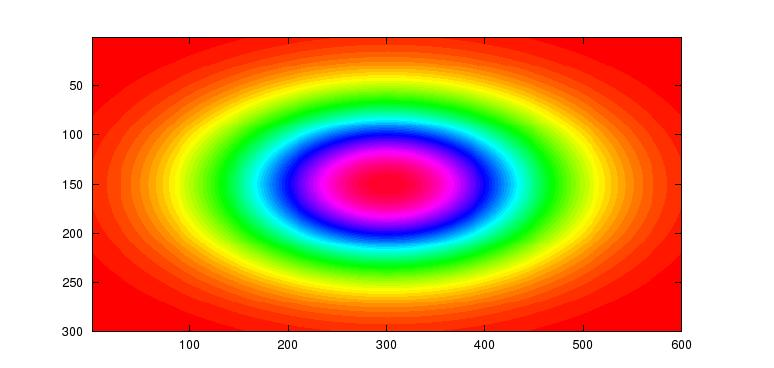
\includegraphics[width=8cm]{zoom1}}


At this point, resizing the window accomplishes nothing, as with a zoom factor 
greater than zero, the size of the image is fixed.

If we change the zoom to another factor larger than 1, we enlarge the image by
the specified factor (or shrink it, for zoom factors \verb|0 < x < 1|.  Here is the
same image zoomed out to 60%
@>


\centerline{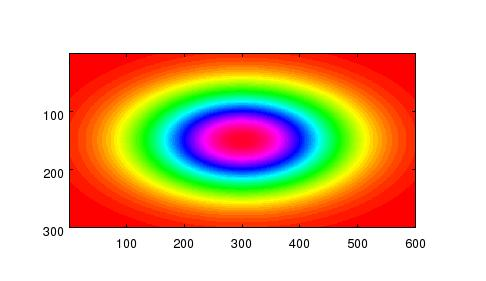
\includegraphics[width=8cm]{zoom3}}


Similarly, we can enlarge it to 130%
@>


\centerline{\includegraphics[width=8cm]{zoom4}}


The ``free'' zoom of \verb|x = 0| results in the image being zoomed to fit the window
without changing the aspect ratio.  The image is zoomed as much as possible in
one direction.
@>


\centerline{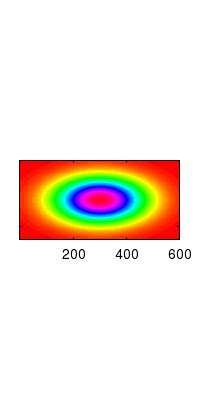
\includegraphics[width=8cm]{zoom5}}


The case of a negative zoom \verb|x < 0| results in the image being scaled arbitrarily.
This allows the image aspect ratio to be changed, as in the following example.
@>


\centerline{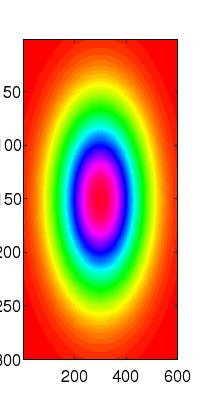
\includegraphics[width=8cm]{zoom6}}

